\subsection{Residual registration}\label{ssec:registration}

Image registration is a fundamental problem in image processing. The aim is to
align two or more images of the same scene often taken at different times, from
different viewpoints, or by different sensors. It is a basic step for
orthorectification, image stitching, image fusion, change detection\ldots
But this process is also critical for stereo reconstruction process to be able
to obtain an accurate estimation of epipolar geometry.

Sensor model is generally not sufficient to provide image registrations. Indeed,
several sources of geometric distortion can be contained in optical remote
sensing images including earth rotation, platform movement, non linearity\ldots

They result in geometric errors on scene level, image level and pixel level. It
is critical to rectify the errors before a thematic map is generated, especially
when the remote sensing data need to be integrated together with other GIS data.

This figure illustrates the generic workflow in the case of image series registration:
%add figure
\begin{center}
     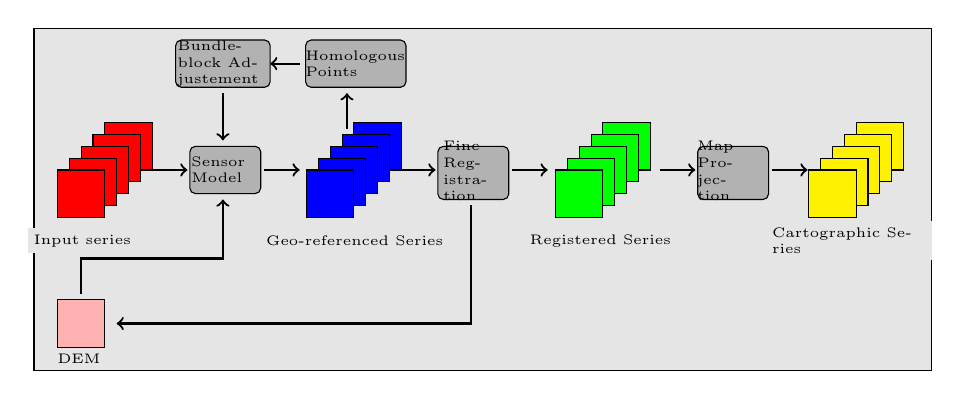
\begin{tikzpicture}[scale=0.15]
    \tiny
    \draw[fill=black!10] (-1,-12) rectangle (75,17);
     \foreach \x in {5,...,1}
       \draw[fill=red] (\x,\x) rectangle +(4,4);
     \node[fill=black!10, text width= 1.5cm] (InputSeries) at
       (4,-1) {Input series};
     %\pause
     \draw[->,thick] (9,5) --  +(3,0);
     %%\pause
     \draw[fill=black!30,rounded corners=2pt] (12.2,3) rectangle +(6,4);
     \node[text width= 0.8cm] (SensorModel) at (15,5) {Sensor Model};
     %\pause
     \draw[fill=red!30] (1,-10) rectangle +(4,4);
     \node[fill=black!10, text width= 1.2cm] (DEM) at
       (5,-11) {DEM};
     %\pause
     \draw[->,thick] (3,-5.5) --  ++(0,3) -- ++(12,0) -- ++(0,5);
     %\pause
     \draw[->,thick] (18.5,5) --  +(3,0);
     %\pause
     \foreach \x in {5,...,1}
       \draw[fill=blue,xshift=600pt] (\x,\x) rectangle +(4,4);
     \node[fill=black!10, text width= 2.8cm] (GeoRefSeries) at
       (28,-1) {Geo-referenced Series};
%\pause


       \draw[->,thick] (25.5,8.5) --  +(0,3);

     \draw[fill=black!30,rounded corners=2pt] (22,12) rectangle +(8.5,4);
     \node[text width= 1.5cm] (HomPoExtr) at (27,14) {Homologous Points};

     \draw[->,thick] (21.5,14) --  +(-2.5,0);

     \draw[fill=black!30,rounded corners=2pt] (11,12) rectangle +(8,4);
     \node[text width= 1.3cm] (BBAdj) at (15.5,14) {Bundle-block Adjustement};

     \draw[->,thick] (15,11.5) --  +(0,-4);

     %\pause
      \draw[->,thick] (30,5) --  +(3,0);
      %\pause
     \draw[fill=black!30,rounded corners=2pt] (33.2,2.5) rectangle +(6,4.5);
     \node[text width= 0.7cm] (FineRegistration) at (36,4.9) {Fine Registration};
     %\pause


     \draw[->,thick] (39.5,5) --  +(3,0);
     %\pause
     \foreach \x in {5,...,1}
       \draw[fill=green,xshift=1200pt] (\x,\x) rectangle +(4,4);
     \node[fill=black!10, text width= 1.8cm] (RegistSeries) at
       (47,-1) {Registered Series};
     %\pause
     \draw[->,thick] (36,2) --  ++(0,-10) -- ++(-30,0);

     %\pause
      \draw[->,thick] (52,5) --  +(3,0);
      %\pause
     \draw[fill=black!30,rounded corners=2pt] (55.2,2.5) rectangle +(6,4.5);
     \node[text width= 0.7cm] (CartoProjection) at (57.5,4.9)
          {Map Projection};
     %\pause


     \draw[->,thick] (61.5,5) --  +(3,0);
     %\pause
     \foreach \x in {5,...,1}
       \draw[fill=yellow,xshift=1810pt] (\x,\x) rectangle +(4,4);
     \node[fill=black!10, text width= 1.95cm] (CartoSeries) at
       (68,-1) {Cartographic Series};


     \end{tikzpicture}
     \end{center}


We will now illustrate this process by applying this workflow to register two
images. This process can be easily extended to perform image series
registration.

The aim of this example is to describe how to register a Level 1 QuickBird image
over an orthorectify Pleiades image over the area of Toulouse, France.


\begin{figure}[!h]
  \center
  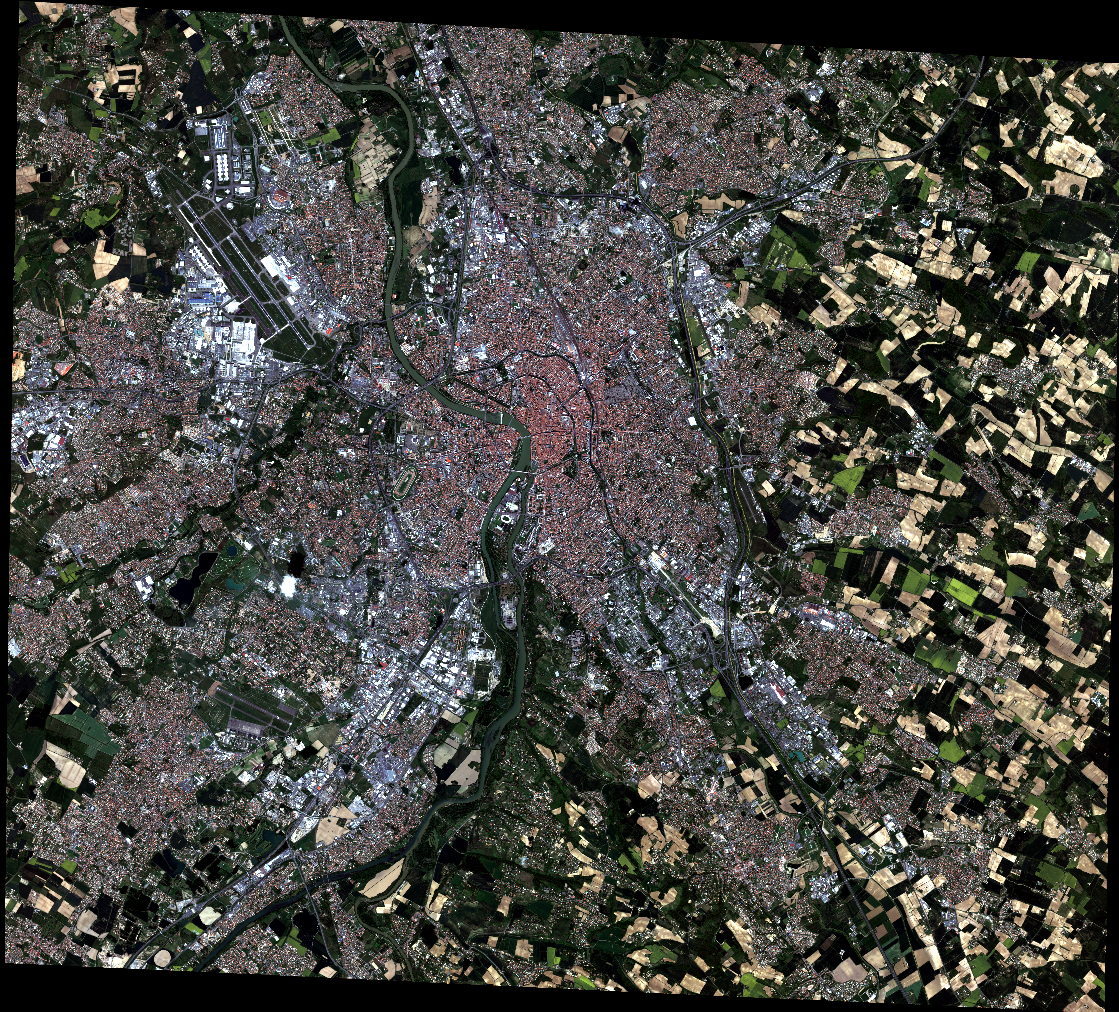
\includegraphics[width=0.45\textwidth]{../Art/MonteverdiImages/registration_pleiades_ql.png}
  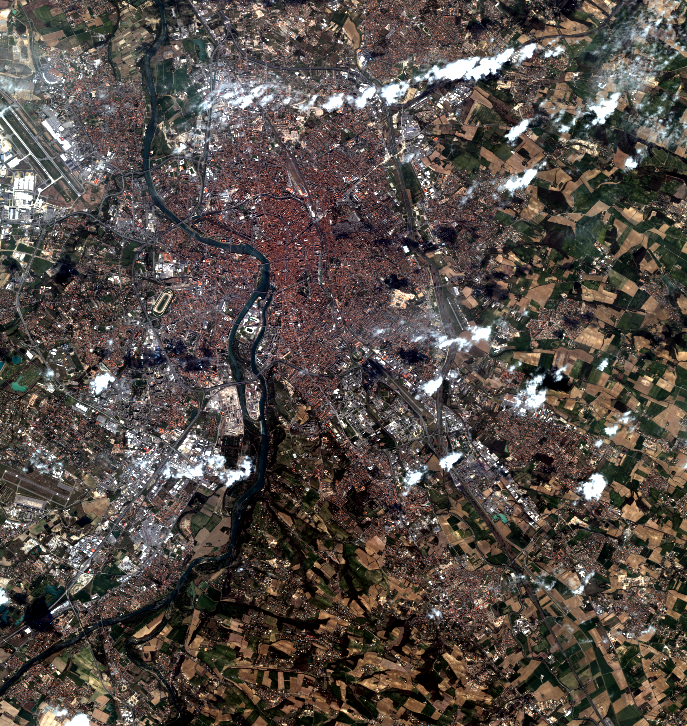
\includegraphics[width=0.45\textwidth]{../Art/MonteverdiImages/registration_quickbird_ql.png}
  \itkcaption[InputImagesRegistration]{From left to right: Pleiades ortho-image, and original QuickBird image over Toulouse}
  \label{fig:InputImagesRegistration}
\end{figure}


\subsubsection{Extract metadata from the image reference}

We first dump geometry metadata of the image we want to refine in a text
file. In OTB, we use the extension \textit{.geom} for this type of file. As you
will see the application which will estimate a refine geometry only needs as
input this metadata and a set of homologous points. The refinement application
will create a new \textit{.geom} file containing refined geometry parameters
which can be used after for reprojection for example.

The use of external \textit{.geom} file is available in OTB since release
$3.16$. See
\href{http://wiki.orfeo-toolbox.org/index.php/ExtendedFileName}{here} for more
information.

\begin{verbatim}

otbcli_ReadImageInfo   -in slave_image
                       -outkwl TheGeom.geom

\end{verbatim}


\subsubsection{Extract homologous points from images}

The main idea of the residual registration is to estimate an second
transformation (after the application of sensors model).

The homologous point application use interest point detection method to get a
set of point which match in both images.

The basic idea is to use this set of homologous points and estimate with them a
residual transformation between the two images.

There is a wide variety of keypoint detector in the literature. They allow to
detect and describe local features in images. These algorithms provide for each
interesting point a ``feature description''. This descriptor has the property to
be invariant to image translation, scaling, and rotation, partially invariant to
illumination changes and robust to local geometric distortion.  keypoints.
Features extracted from the input images are then matched against each
other. These correspondences are then used to create the homologous points.

\href{http://en.wikipedia.org/wiki/Scale-invariant_feature_transform}{SIFT} or
\href{http://en.wikipedia.org/wiki/SURF}{SURF} keypoints can be computed in the
application. The band on which keypoints are computed can be set independently
for both images.

The application offers two modes :
\begin{itemize}
\item the first is the full mode where keypoints
are extracted from the full extent of both images (please note that in this mode
large image file are not supported).
\item The second mode, called \textit{geobins},
allows to set-up spatial binning so as to get fewer points spread across the
entire image. In this mode, the corresponding spatial bin in the second image is
estimated using geographical transform or sensor modeling, and is padded
according to the user defined precision.
\end{itemize}

Moreover, in both modes the application can filter matches whose co-localization in
the first image exceed this precision. Last, the elevation parameters allow to deal
more precisely with sensor modelling in case of sensor geometry data. The
\textit{outvector} option allows to create a vector file with segments
corresponding to the localization error between the matches.

Finally, with the \textit{2wgs84} option, you can match two sensor geometry images or a
sensor geometry image with an ortho-rectified reference. In all cases, you get
a list of ground control points spread all over your image.

\begin{verbatim}


otbcli_HomologousPointsExtraction   -in1 slave_image
                                    -in2 reference_image
                                    -algorithm surf
                                    -mode geobins
                                    -mode.geobins.binstep 512
                                    -mode.geobins.binsize 512
                                    -mfilter 1
                                    -precision 20
                                    -2wgs84 1
                                    -out homologous_points.txt
                                    -outvector points.shp
                                    -elev.dem dem_path/SRTM4-HGT/
                                    -elev.geoid OTB-Data/Input/DEM/egm96.grd

\end{verbatim}

Note that for a proper use of the application, elevation must be correctly set
(including DEM and geoid file).

\subsubsection{Geometry refinement using homologous points}

Now that we can use this set of tie points to estimate a residual
transformation.For this we use the dedicated application called
\textbf{RefineSensorModel}. This application make use of OSSIM capabilities to
align the sensor model.

It reads the input geometry metadata file (\textit{.geom}) which contains the
sensor model information that we want to refine and the text file
(homologous\_points.txt) containing the list of ground control point. It
performs a least-square fit of the sensor model adjustable parameters to these
tie points and produces an updated geometry file as output (the extension which
is always use is \textit{.geom})

The application can provide as well an optional ground control points based
statistics file and a vector file containing residues that you can display in a
GIS software.

Please note again that for a proper use of the application, elevation must be
correctly set (including DEM and geoid file). The map parameters allows to
choose a map projection in which the accuracy will be estimated (in meters).

Accuracy values are provided as output of the application (computed using tie
points location) and allow also to control the precision of the estimated model.

\begin{verbatim}

otbcli_RefineSensorModel   -elev.dem dem_path/SRTM4-HGT/
                           -elev.geoid OTB-Data/Input/DEM/egm96.grd
                           -ingeom slave_image.geom
                           -outgeom refined_slave_image.geom
                           -inpoints homologous_points.txt
                           -outstat stats.txt
                           -outvector refined_slave_image.shp

\end{verbatim}

\subsubsection{Orthorecrtify image using the affine geometry}

Now we will show how we can use this new sensor model. In our case we'll use
this sensor model to orthorectify the image over the Pléiades reference. \otb
offers since version 3.16 the possibility to use
href{http://wiki.orfeo-toolbox.org/index.php/ExtendedFileName}{extend image}
path to use different metadata file as input. That's what we are going to use
there to orthorectify the QuickBird image using the \textit{.geom} file obtained
by the \textbf{RefineSensorModel} applications.  over the first one using for
the second image estimated sensor model which take into account the original
sensor model of the slave and which also fit to the set of tie points.

\begin{verbatim}

otbcli_OrthoRectification   -io.in slave_image?&geom=TheRefinedGeom.geom
                            -io.out ortho_slave_image
                            -elev.dem dem_path/SRTM4-HGT/
                            -elev.geoid OTB-Data/Input/DEM/egm96.grd
                     
\end{verbatim}

As a result, if you've got enough homologous points in images and control that
the residual error between the set of tie points and the estimated sensor model
is small, you must achieve a good registration now between the 2 rectified
images. Normally far better than 'only' performing separate orthorectification
over the 2 images.

This methodology can be adapt and apply in several cases, for example :
\begin{itemize}

\item register stereo pair of images and estimate accurate epipolar geometry
\item registration prior to change detection

\end{itemize}
